\section{Analysis of multiple datasets --- ``metafile processing''}
\label{sec:level2}

\purplebox{}
It is assumed that you have processed multiple NanoSIMS datasets using steps described in Section~\ref{sec:level1}, which left you with output such as isotope ratio values and images scatterred across \bb{multiple} files and folders, organized as described in Section~\ref{sec:data_organization}. This section explains how to quickly \bb{merge} these multiple files into \bb{one} output. This output, and in particular the isotope ratio values exported in a~text format, can be used for further, more sophisticated analyses (e.g., statistical analysis) by other, third-party software. If you are a~skilled data analyst, you can arguably do this more efficiently by creating scripts in a~programming language of your choice. This section describes how to do this in LANS, if your coding abilities are more limited.
\tcbe

As an example, we will use processed data for four datasets, each corresponding to cyanobacterial cells incubated under different experimental conditions (treatments): 
\begin{itemize}
\item[--]\ttt{2018-01-05-GAP2017\_1} (treatment~0)
\item[--]\ttt{2018-01-05-GAP2017\_2} (treatment~1)
\item[--]\ttt{2018-01-11-GAP2017\ 3} (treatment~2)
\item[--]\ttt{2018-01-11-GAP2017\_5} (treatment~3)
\end{itemize}
The datasets and the corresponding folders containing the processed data (backed up in \ttt{zip} files, as described in Section~\ref{sec:final-steps}, step~3) are available in the same location as the LANS program (folder \ttt{test\_data/GAP2017}). It is recommended that you check these data before you continue with the metafile processing steps described in this section.

%%%%

\subsection{Generate metafile}
\setcounter{step}{0}

\goldbox{}
The first step involves the definition of a~list of datasets and variables that you want to merge and analyze together. In the context of LANS, this list is stored in a~so-called \bb{metafile}, which is a~simple text file containing the required information including the absolute path to the processed data structure, relative paths for the individual datasets, and variables of interest (see below, step~10). This file can be generated in a~simple text editor, but it is better to start using a~dedicated tool in LANS to avoid syntax or formatting errors.
\tcbe

\s{Back in the main LANS window, select \lans{Process multiple} $\ra$ \lans{Generate metafile} to open a~new tool window dedicated to metafile definition (Fig.~\ref{fig:metafile-definition}). }

\begin{figure}[!ht]
\centering
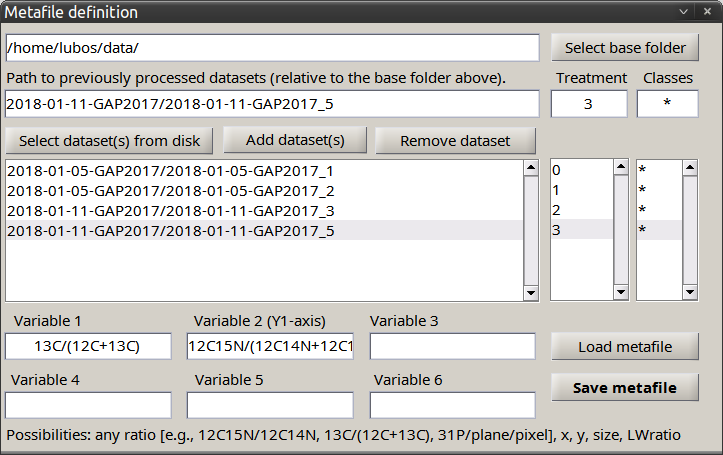
\includegraphics[scale=0.4]{figs3/LANS-metafile-definition}
\caption{\label{fig:metafile-definition}%
LANS tool for defining a~metafile.}
\end{figure}

\s{In this tool window, click on \lans{Select base folder} to select the absolute path to the processed datasets.}

\nb{It is assumed that the folders with the processed datasets are located in this path or in sub-folders under it.}

\s{Click on \lans{Select dataset(s) from disk}, navigate to a~specific processed dataset, and select it.}

\nb{You need to select the raw data file (\ttt{im} or \ttt{im.zip} file), not the sub-folder containing the processed data. However, the corresponding sub-folder with the processed data must exist.}

\nnb{You can select multiple datasets at once by holding the \ttt{Ctrl} key while selecting the files.}

\nnb{You can also select the \ttt{prefs.mat} file corresponding to the raw dataset. If you processed the dataset and stored the preferences at the end of processing, as emphasized in Section~\ref{sec:final-steps}, step~2, this file will be present in the dataset folder.}

\s{Enter a~\lanstf{treatment identifier} to the provided field.}

\nb{This must be an \bb{integer number}, e.g., $0$ for a~control treatment, $1$ for treatment~1, etc.}

\nnb{It is up to you to keep track of the correspondence between the treatment identifiers and the true meaning of the treatments.}

\s{Enter \lanstf{ROI classes} to the provided field.}

\nb{Enter \ttt{*} if you want to analyze \bb{all} ROI classes, unless you really only want to analyze ROIs from a~specific class. Note that you will be able to make this selection later on anyway, so it is best to simply enter \ttt{*}.}

\s{Click \lans{Add dataset(s)} to add the dataset(s) to the list. }

\s{Repeat steps 3--6 to select all datasets that should be part of the metafile processing.}

\nb{If you want to remove a dataset from the list, select it in the list and then click \lans{Remove dataset}.}

\s{In the fields provided, enter \lanstf{variables} that you want to analyze via metafile processing. }

\nb{Ensure that you type the strings \emph{exactly} in the same way as you did during the processing of individual datasets (e.g., \ttt{13C/12C}, \ttt{13C/(12C+13C)}, \ttt{12C15N/12C14N}, \ttt{31P/plane/pixel}, etc.). Best is to copy and paste the strings from the main LANS window to avoid typos.}

\nnb{You can analyze up to six variable simultaneously. The idea behind this limit is that you can, later on, plot the variables against each other in up to three 2D-scatter plots or up to two 3D-scatter plots. Thus, it is good to think ahead and enter the variables in the order how you want to plot them later on, e.g., \ttt{13C/12C} as variable~1 (later $x$), \ttt{12C15N/12C14N} as variable~2 (later $y$), etc.}

\s{Click \lans{Save metafile} and define the name and location for the metafile.}

\nb{Ideally, to keep everything well organized, the metafile should be located in the \lanstf{base folder} selected above. }

\nnb{For example, if you call the metafile \ttt{m1.txt}, any output generated during processing of this metafile will be stored in a~sub-folder called \ttt{m1}.}

\s{Optionally, explore the content of the metafile by opening it in a~simple text editor (e.g., \ttt{notepad} or \ttt{notepad++}).}

\nb{This is recommended because, later on, you may find it easier to edit the content of this file (e.g., add or remove datasets, modify the variables) directly in the editor rather than through steps 2--8 described above. An example of the metafile content is shown here:
\begin{center}
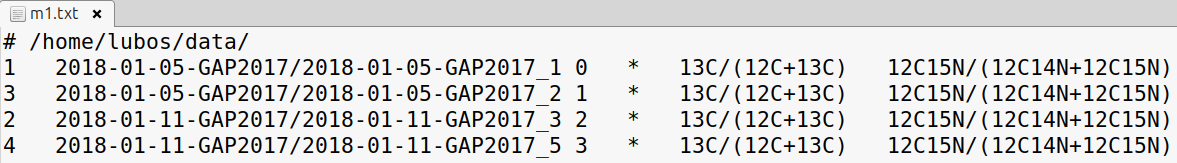
\includegraphics[scale=0.35]{figs3/LANS-metafile-m1}
\end{center}}

%%

\subsection{Process metafile}
\setcounter{step}{0}

\goldbox{}
First, we describe steps that are common for different types of metafile processing analysis available in LANS. Subsequent steps depend on the particular analysis you want to perform and are described in separate sections below.
\tcbe

\s{Ensure that the metafile is defined and the sub-folders and corresponding output files exist and are consistent for all datasets listed in the metafile.}

\nb{This should be the case if you conducted the data processing attentively and in accordance with instructions described in Section~\ref{sec:level1}. If there are inconsistencies, they will be reported later on in the console (see below).}

\s{In the main LANS window, select \lans{Process multiple} $\ra$ \lans{Process metafile} to open a~new tool window dedicated to metafile processing (Fig.~\ref{fig:process-metafile}).}

\begin{figure}[!ht]
\centering
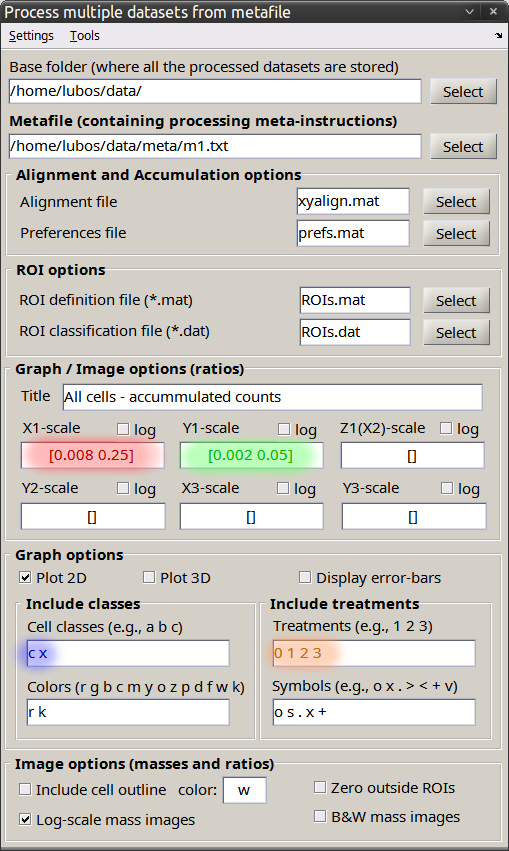
\includegraphics[scale=0.4]{figs3/LANS-process-metafile}
\caption{\label{fig:process-metafile}%
LANS tool for processing a~metafile. If the scale of the variable is specified (highlighted in red and green), it will be applied in the subsequent analyses. An empty scale (\ttt{[]}) will have no effect. In the areas highlighted by blue and orange, you can specify the ROI classes and treatments that should be displayed in the scatter plots, respectively.}
\end{figure}

\s{In this tool window, select the \lanstf{base folder}.}

\nb{Typically, this folder will be the same as specified during metafile definition. However, if you reorganized the data on your computer, or if you conduct the metafile processing on a~different computer, the data organization may be quite different. Thus, this feature makes the metafile processing portable across different computers.}

\s{Select the \lanstf{metafile}.}

\s{Specify  the \lanstf{scale}, separately for each variable.}

\nb{If specified in the form of \ttt{[min max]}, corresponding to a~minimum and maximum value, the scale will be applied during the following analyses. For example, images for the corresponding variable will be reexported as PDF using this new scale, or scatter plots containing the variable will apply this new scale.}

\nnb{However, since the optimal scale for the images or graphs may initially be unknown, it is a~good idea to start with an empty scale, indicated by \ttt{[]}. This will have no effect on the displayed graphs or images for the corresponding variable.}

\s{Check \lanscb{log} if you want the variable to be log-transformed before display.}

\nb{This can be done separately for each variable.}

\s{Specify the mapping between ROI classes and \lanstf{colors} and between treatments and \lanstf{symbols} in the respective fields. }

\nb{This mapping will be applied when plotting scatter plots.}

\nnb{Colors and symbols recognized by Matlab are already listed between the parentheses (e.g., colors: \ttt{r} for red, \ttt{g} for green, \ttt{b} for blue, \ttt{k} for black, etc., symbols: \ttt{o} for circles, \ttt{s} for squares, \ttt{x} for crosses, \ttt{.} for points, etc.).}

\s{Save the metafile processing settings using \lans{Settings} $\ra$ \lans{Save settings}.}

\nb{This is useful if you plan to return to the same metafile processing session in the future.}

\nnb{Previously saved settings can be loaded using \lans{Settings} $\ra$ \lans{Load settings}.}

\nnb{Now you are ready to continue with different types of metafile processing analyses, using steps described in the following sections.}

\subsubsection{Export images for selected variables}
\label{sec:621}
\setcounter{step}{0}

\goldbox{}
This section describes how to merge \bb{images} from multiple datasets into one graphical output (PDF), separately for each variable in the metafile (example shown in Fig.~\ref{fig:metafile-images}). This output is useful for quality checking of ROI definitions and visual assessment or comparative analysis of ion count and ratio images.
\tcbe

\s{In the Process metafile window, enter the \lanstf{ROI definition file} in the corresponding field.}

\nb{This is only relevant if you want to include ROIs in reexported images.}

\nnb{It is important that the ROI definition files have the \emph{same name} for \emph{all} datasets in the metafile (e.g., \ttt{ROIs.mat} or \ttt{cells.mat}). This explains why you need to use consistently the same filename when defining ROIs during the analysis of individual datasets.}

\s{Select \lans{Tools} $\ra$ \lans{Export images for each variable as PDF}, or press \ttt{Ctrl+m}. }

\nb{This step will combine images of the variables from multiple datasets and export them in a~PDF output, \bb{one file per variable}, allowing you to view all images from a~specific project in one place.}

\nnb{The visual comparison of images can be made easier if all images are displayed in the same scale. This is achieved by setting the minimum and maximum values in the corresponding \lanstf{scale} field, as explained above. If you specify the scale, formatted as \ttt{[min max]}, all images of the corresponding variable will be reexported as PDF using the new scale (Fig.~\ref{fig:process-metafile}). If you do not want to reexport the images (e.g., because you have already done so earlier), you need to set the corresponding scale back to \ttt{[]} (i.e., an empty vector).}

\nnb{When doing this, you can use the \lanscb{log} checkbox to set whether a~log-transformed data should be displayed, or the \lanscb{Include ROI outlines} checkbox to set whether the ROI outlines should be included. For the ROI outlines, you can also specify their \lanstf{color} in the corresponding field (e.g., \ttt{w} for white) (Fig.~\ref{fig:process-metafile}). }

\nnb{Observe the console for possible error messages, which are issued if a~particular file is missing. It may be that there is a~typo in the metafile, or that you forgot to export the variable for a~particular dataset. If this is the case, you will need to reanalyze that dataset and fix the issue.}

\nnb{Observe the console to see the exact locations of the output created by this action. For example, if your metafile is called \ttt{m1.txt} and the variables of interest include \ttt{13C/(12C+13C)} and \ttt{12C15N/(12C14N+12C15N)}, the images will be exported in files called \ttt{13C-(12C+13C).pdf} and \ttt{12C15N-(12C14N+12C15N).pdf}, respectively, located in the sub-folder \ttt{m1} of the \lanstf{base folder}. Note that the use of \ttt{-} in place of \ttt{/} is necessary because the latter symbol is reserved as a~folder separator in the absolute path to files.}

\nnb{Example of the output generated by these steps is shown in Fig.~\ref{fig:metafile-images}.}

\begin{figure}[!ht]
\centering
\begin{tabular}{cc}
(A) & (B) \\
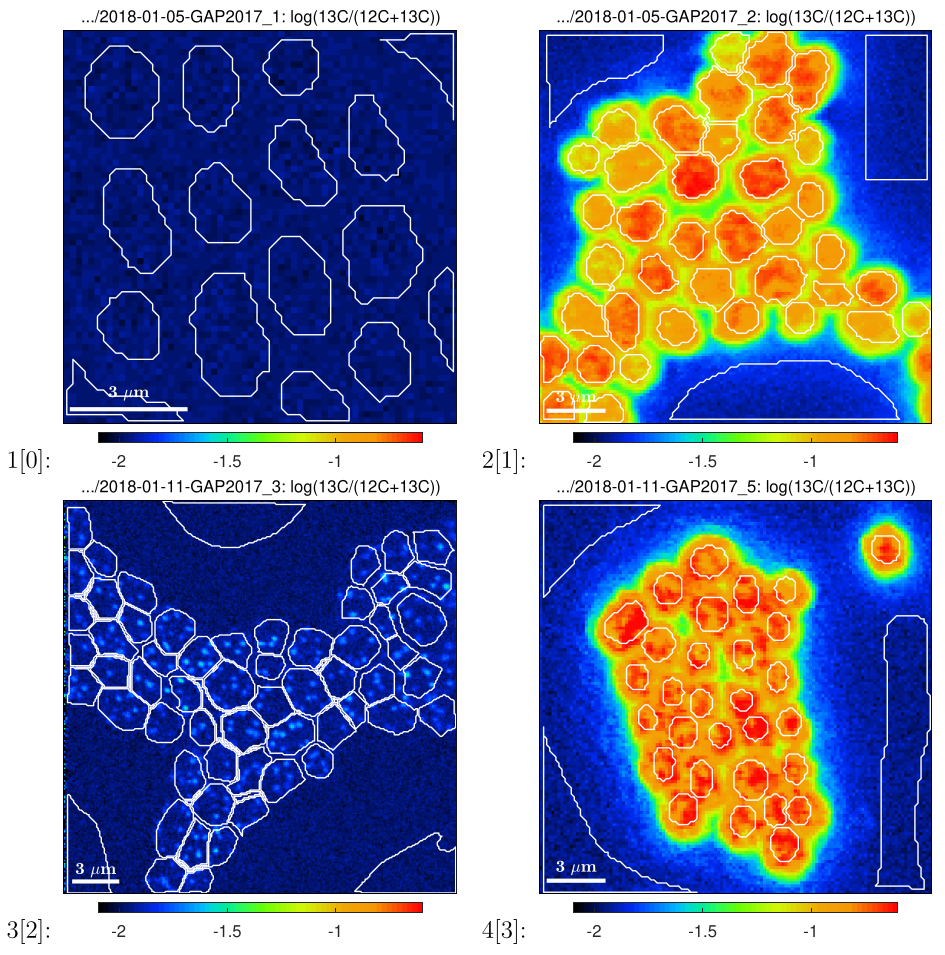
\includegraphics[width=0.47\textwidth, valign=t]{figs3/log(13C-(12C+13C))}
&
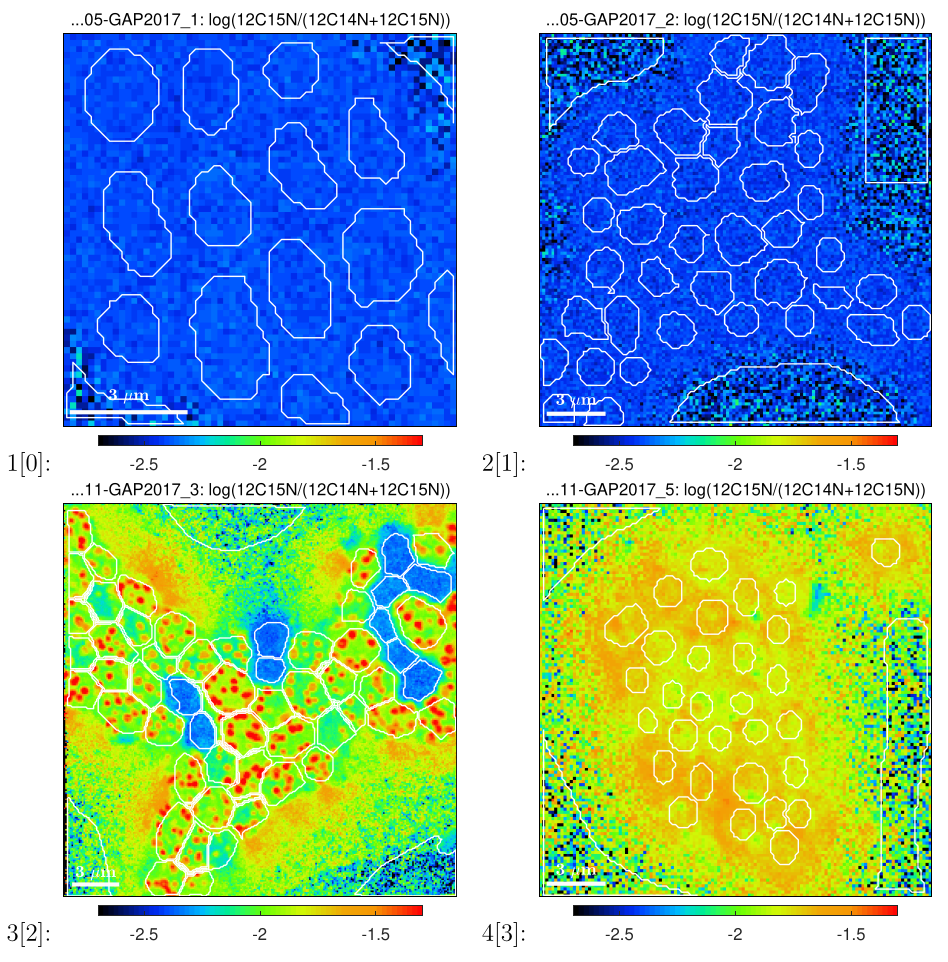
\includegraphics[width=0.47\textwidth, valign=t]{figs3/log(12C15N-(12C14N+12C15N))}
\end{tabular}
\caption{\label{fig:metafile-images}%
Example of the output generated by metafile processing. Shown are (A) \ttt{13C/(12C+13C)} and (B) \ttt{12C15N/(12C14N+12C15N)} ratio images for four datasets. ROI outlines corresponding to individual cells are included, allowing you to quality-check the ROI definition across all datasets. Images have been log-transformed to allow simultaneous visualization of low and high values. All images for a~particular variable are shown in the same scale to aid visual comparison among treatments. The treatment identifiers are shown between brackets ([0--3]) at the bottom-left of each image.}
\end{figure}

%%%%

\subsubsection{Export ROI-specific data for selected variables}
\label{sec:622}
\setcounter{step}{0}

\goldbox{}
This section describes how to merge \bb{text output} from multiple datasets into one data file. The output contains ROI-specific information generated by the analyses of individual datasets, including values of ion counts and ion count ratios, Poisson errors, ROI positions, sizes and classes, and treatment identifiers. This type of information can further be analyzed by statistical tools offerred by LANS (see next section) and beyond.
\tcbe

\s{In the Process metafile window, enter the \lanstf{ROI definition file} in the corresponding field.}

\nb{It is important that the ROI definition files have the \emph{same name} for \emph{all} datasets in the metafile (e.g., \ttt{ROIs.mat} or \ttt{cells.mat}). This explains why you need to use consistently the same filename when defining ROIs during the analysis of individual datasets.}

\s{Enter the \lanstf{ROI classification file} in the corresponding field.}

\nb{This is only relevant if you want to plot ROIs from different classes in different colors.}

\nnb{Similar to the ROI definition files, the ROI classification files must have the \emph{same name} for \emph{all} datasets in the metafile (e.g., \ttt{ROIs.dat} or \ttt{cells.dat}). This explains why you need to use consistently the same filename when classifying ROIs during the analysis of individual datasets.}

\s{Select checkboxes in the \ttt{Graph options} box to specify whether you want to plot a~\lanscb{2D} scatter plot or a~\lanscb{3D} scatter plot, or whether you want to include \lanscb{error-bars} for each data-point.}

\nb{When plotting 2D scatter plots, 2, 4 or 6 variables must be specified in the metafile. When plotting 3D scatter plots, 3 or 6 variables must be specified in the metafile. }

\nnb{When including error-bars, Poisson error is used as the size of the error-bar.}

\s{Select \lans{Tools} $\ra$ \lans{Export and display data in ROIs} $\ra$ \lans{For all datasets in one graph}, or press \ttt{Ctrl+p}.}

\nb{This step will \bb{merge} ROI-specific data, such as ion counts or ion count ratios, from \bb{multiple} datasets and export the results in \bb{one} data file (with an~extension \ttt{dac}). This file is probably the most useful output for your project, if the project conclusions are drawn from ROI-specific data derived from the analysis of multiple NanoSIMS datasets.}

\nnb{In addition to merging and exporting the data, this step will also \bb{plot} the ROI-specific values in a~scatter plot (2D or 3D), using different colors and symbols for different ROI classes and treatments (Fig.~\ref{fig:metafile-scatterplot}).}

\begin{figure}[!b]
\centering
\begin{tabular}{cc}
(A) & (B) \\
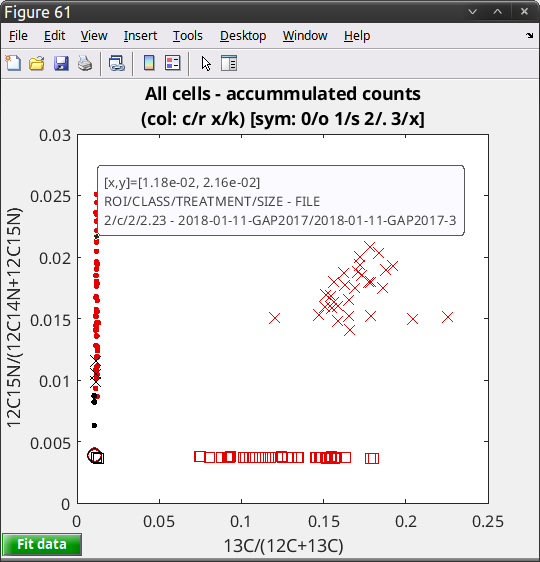
\includegraphics[width=0.44\textwidth, valign=t]{figs3/LANS-metafile-scatterplot1}
&
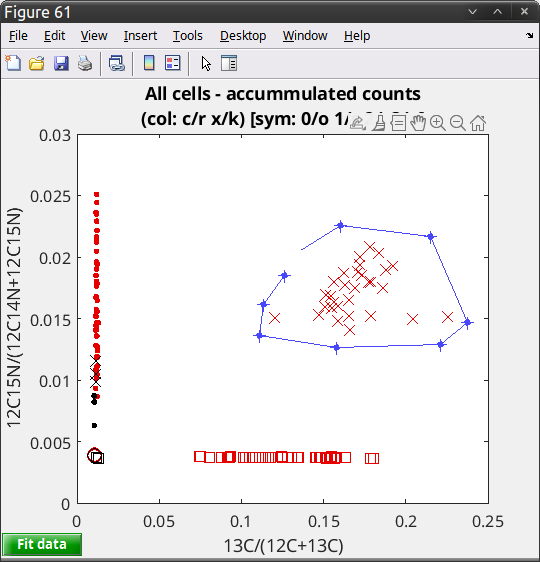
\includegraphics[width=0.44\textwidth, valign=t]{figs3/LANS-metafile-scatterplot2}
\end{tabular}
\caption{\label{fig:metafile-scatterplot}%
Example of a~scatter plot generated by metafile processing.  The plot shows data from four datasets, each corresponding to a~different treatment. (A) By clicking on a~particular data point, you can quickly view relevant information about the data point and thus trace it to a~particular dataset. (B) By clicking on the \lans{Fit data} button, you can manually select a~set of data points (by enclosing them in a~polygon) and analyse them using various types of statistical analyses, including linear regression. }
\end{figure}

\nnb{This scatter plot allows you to quickly assess the ROI-specific data visually. It also offers several useful functions to check the data quality and consistency. For example, if you click with a~mouse on a~particular data point, an annotation will appear providing relevant information about the data point (e.g., the source dataset, ROI identifier, ROI class; Fig.~\ref{fig:metafile-scatterplot}A). You can also click on the \lans{Fit data} button to quickly perform various types of basic statistical analyses on manually selected data points, including linear regression (Fig.~\ref{fig:metafile-scatterplot}B).}

\nnb{When merging data from multiple datasets, observe the console for possible error messages, which are issued if a~particular file is missing. It may be that there is a~typo in the metafile, or that you forgot to export the data for a~particular dataset. If this is the case, you will need to reanalyze that dataset and fix the issue.}

\nnb{Observe the console to see the exact locations of the output created by this action. For example, if your metafile is called \ttt{m1.txt} and the variables of interest include \ttt{13C/(12C+13C)} and \ttt{12C15N/(12C14N+12C15N)}, the ROI-specific data will be exported in the file called \ttt{m1.dac} and the scatter plot will be exported in the file called \ttt{m1-13C-(12C+13C)--12C15N-(12C14N+12C15N)-all.pdf}, both located in the sub-folder \ttt{m1} of the \lanstf{base folder}.}

%%

\subsubsection{Basic statistical analysis}

\goldbox{}
Statistical analysis of ROI-specific data for a particular project can be done by third-party tools using the text output generated as described in the previous section.  However, if your statistical knowledge and skills are limited, you can perform some \bb{basic} analyses in LANS, such as calculating group means and standard deviations or comparing means among groups (ROI classes or treatments). The following steps describe how to do this via metafile processing in LANS.
\tcbe

\noindent
The initial 2 steps are the same as those described in the previous section and will not be repeated here.

\setcounter{step}{2}
\s{Select \lans{Tools} $\ra$ \lans{Compare classes and treatments}, or press \ttt{Ctrl+e}.}

\nb{This step will merge ROI-specific data from multiple datasets and pass the output to a~tool that allows you to perform the statistical analysis (Fig.~\ref{fig:lans-statistics}).}

\s{Select multiple checkboxes for the \lanscb{ROI classes}, then select one checkbox for the \lanscb{Treatment} of interest,  and then select \lans{Compare} $\ra$ \lans{Classes} (Fig.~\ref{fig:lans-statistics}A).}

\nb{This selection will allow you to compare values across multiple ROI classes for one specific treatment.}

\s{Select the \lans{Test type} and the \lans{Ratio} you want to analyze.}

\nb{For example, by selecting Levene's test and \ttt{13C/(12C+13C)}, you will be able to test for the homogeneity of variance in the ${}^{13}C$ atom fractions.}

\s{Click on \lans{Run test} to perform the analysis. }

\nb{Results will be displayed in the graph (Fig.~\ref{fig:lans-statistics}A) and also in the Matlab console.}

\begin{figure}[!th]
\centering
\begin{tabular}{cc}
(A) & (B) \\
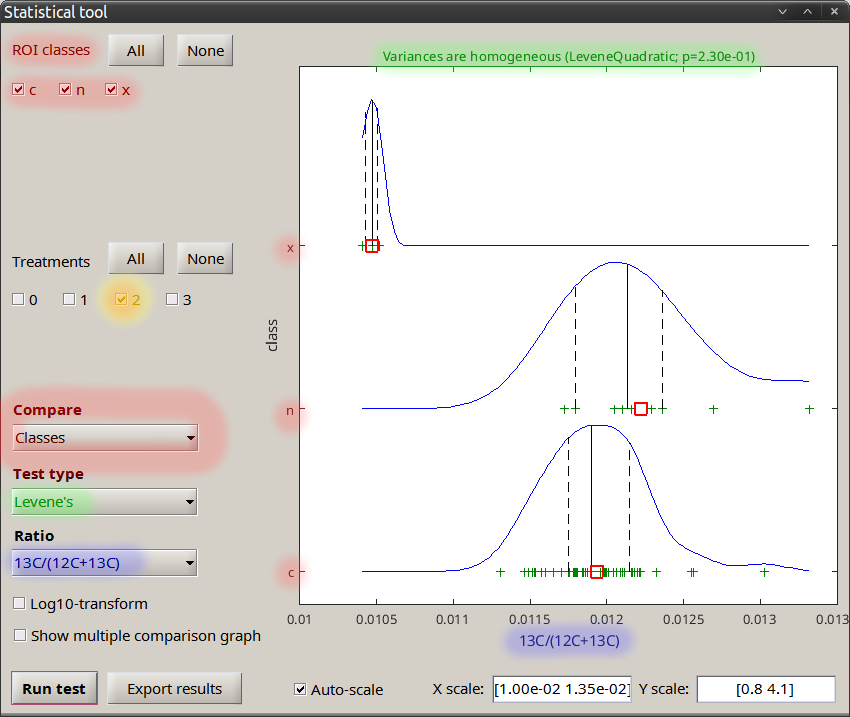
\includegraphics[width=0.48\textwidth, valign=t]{figs3/LANS-statistics1}
&
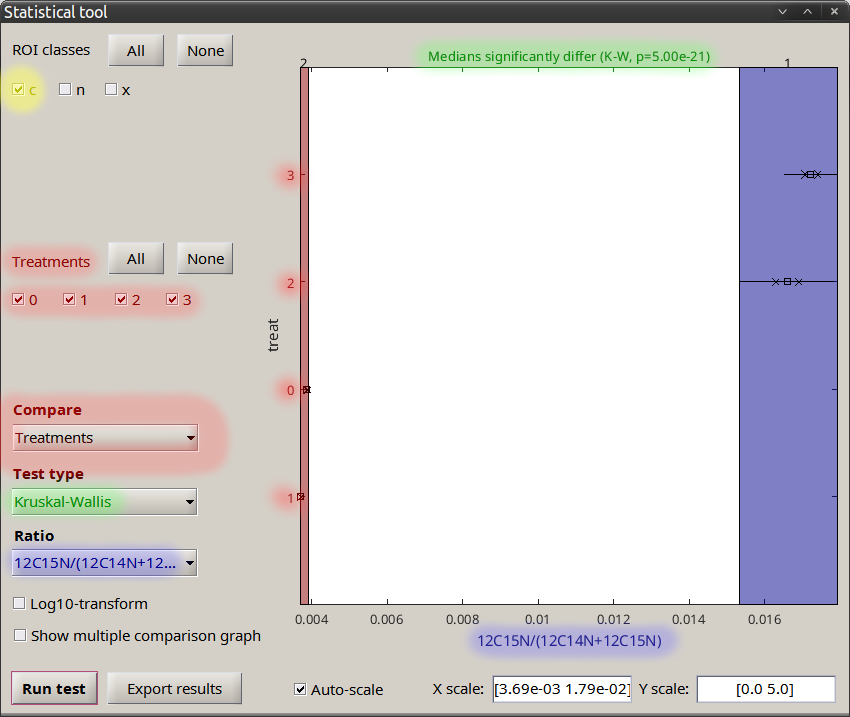
\includegraphics[width=0.48\textwidth, valign=t]{figs3/LANS-statistics2}
\end{tabular}
\caption{\label{fig:lans-statistics}%
Examples of basic statistical tests that you can perform in LANS. (A) Comparison of multiple classes for one treatment. (B) Comparison of multiple treatments for one class. Note the relationships between the fields highlighted in the same color.}
\end{figure}

\s{Click on \lans{Export results} to export the results as text and graphics.}

%%

\s{Select multiple checkboxes for the \lanscb{Treatments}, then select one checkbox for the \lanscb{ROI class} of interest,  and then select \lans{Compare} $\ra$ \lans{Treatments} (Fig.~\ref{fig:lans-statistics}B).}

\nb{This selection will allow you to compare values across multiple treatments for one specific ROI class.}

\s{Select the \lans{Test type} and the \lans{Ratio} you want to analyze.}

\nb{For example, by selecting Kruskal-Wallis test and \ttt{12C15N/(12C14N+12C15N)}, you will be able to compare median values of the ${}^{15}N$ atom fractions across selected treatments.}

\s{Click on \lans{Run test} to perform the analysis. }

\nb{Results will be displayed in the graph (Fig.~\ref{fig:lans-statistics}B) and also in the Matlab console.}

\nnb{If you additionally select the \lanscb{Show multiple comparison graph} checkbox, you will be able to identify which differences among groups are significant or not.}

\s{Click on \lans{Export results} to export the results as text and graphics.}

%%%%

\subsubsection{Auto-process datasets}
\setcounter{step}{0}

\goldbox{}
Sometimes, it may happen that after you have merged the outputs from multiple datasets for specific variables, you realize that you need a~similar output but for an~\emph{extra} variable, or multiple extra variables, which you have \emph{not} considered when conducting the original analysis of the individual datasets. For example, you have defined ROIs, exported ROI-specific values for the variables \ttt{13C/(12C+13C)} and \ttt{12C15N/(12C14N+12C15N)} and combined them from all datasets in your project, but now you realize that it would also be interesting to check for possible correlations between ROI-specific values of \ttt{31P} and \ttt{16O}. To do this check, you need to export the ROI-specific values for two extra variables: \ttt{31P/plane/pixel} and \ttt{16O/plane/pixel}. 
\tcbe

One option would be to reprocess each individual dataset separately, one by one, using steps described in Section~\ref{sec:level1}. While this would not be a~`big drama' for a~small number of datasets (e.g., 2--3), it could become a~major effort for a~larger number of datasets. To aid this situation, LANS offers a~more convenient solution, accessible via \lans{Tools} $\ra$ \lans{Auto-process datasets}.

\goldbox{}
When performing this action, it is essential that you have done the \bb{minimal} processing of the relevant datasets already, and this processing was done in the \bb{same way} for each dataset. That is, it is expected that for each dataset you have (i) drift-corrected and accumulated the individual planes, (ii) defined and classified ROIs, and (iii) stored the preferences. If you have done this, then the files storing this \bb{minimal information} should be present in the corresponding output sub-folder for each dataset and the auto-processing should run smoothly. If this is not the case for a~specific dataset (e.g., you forgot to store the preferences), you will need to reprocess that dataset first to ensure that the required information \bb{is} stored.
\tcbe

\sbx{Create a new metafile containing the new variables that you want to quantify and later analyze. }

\nb{In this example, you can copy the metafile \ttt{m1.txt} to \ttt{m2.txt} and change all occurances of \ttt{13C/(12C+13C)} and \ttt{12C15N/(12C14N+12C15N)} to \ttt{31P/plane/pixel}	and \ttt{16O/plane/pixel}, respectively. The rest of the metafile remains the same because you want to do the analysis for the same datasets as before.}

\s{Back in the \lans{Process multiple datasets} window, specify the filenames storing the \bb{minimal information} in the corresponding \lanstf{fields}.}

\nb{In most cases, the default filenames will be fine: \ttt{xyalign.mat} for the \lanstf{Alignment file} (the drift-correction information), \ttt{ROIs.mat} and \ttt{ROIs.dat} for the \lanstf{ROI definition file} and \lanstf{ROI classification file}, and \ttt{prefs.mat} for the \lanstf{Preferences file}. }

\nnb{If you have used other filenames, choose those instead. It is important, however, that you have used the \emph{same} filenames for \emph{each} dataset.}

\s{Select the updated \lanstf{metafile}.}

\nb{In this example, it will be \ttt{m2.txt}.}

\s{Select \lans{Tools} $\ra$ \lans{Auto-process datasets}.}

\nb{This step will reprocess \emph{each} dataset in the metafile in the same way as if you processed it yourself, manually, based on the \bb{minimal information} stored in the corresponding files. }

\nnb{Specifically: (i) the raw data will be loaded, (ii) selected planes will be drift-corrected and accumulated for all detected masses (based on the information stored in the preferences and drift-correction files), (iii) the new variables specified in the metafile will be calculated and exported as PDF images, (iv) ROI information will be loaded, and (v) ROI-specific values for the new variables will be calculated and exported in data files. In this particular example, files \ttt{31P-plane-pixel.dac} and \ttt{16O/plane/pixel.dac} will be created in the \ttt{dat} sub-folder for each dataset.}

\sbx{Observe the progress of these processing steps in the Matlab console.}

\nb{If everything goes smoothly and the number of datasets is large, you will have time to make yourself a~cup of tea or coffee and enjoy the moment while LANS is doing the work! }

\nnb{It may happen, however, that the processing encounters an error. For example, if one of the files with the minimal information is missing (this typically happens for files \ttt{prefs.mat} or \ttt{ROIs.mat}), an~error is issued and the auto-processing stops. If this happens, you will need to do two things. First, you need to fix the error by manually processing the relevant dataset again and making sure that the minimal information \emph{is} stored. After doing this, you could start the auto-processing again. But it would be a~waste of time if the reprocessing were done for datasets that had already been reprocessed without errors. To avoid this, you can apply the following trick: open the metafile in a~basic text editor of your choice (e.g., \ttt{notepad} or \ttt{notepad++}, but definitely not a~word-processing program such as \ttt{Word}) and add a~hash symbol (\ttt{\#}) at the very beginning of the line for each dataset that you do \emph{not} want to be reprocessed. Subsequently, save the updated metafile and select \lans{Tools} $\ra$ \lans{Auto-process datasets} to continue with the auto-processing. If an~error occurs again, this time due to a~relevant file missing for another dataset, you need to repeat these steps.}

\nnb{If no errors occurred, you will arrive with an output that will allow you to do the same actions as described above (Sections \ref{sec:621} or \ref{sec:622}), but now with images and data generated also for the extra variables. Before you continue with those actions, do not forget to update the metafile again, this time by \emph{removing} the hash symbols on lines with datasets that you do want to include in your final metafile processing analysis. \bb{Remember:} except for the very first line in the metafile, a~hash symbol at the beginning of a~line means that the corresponding dataset will be ingored during metafile processing.}

\nnb{After performing the steps above, the output generated for the new metafile \ttt{m2.txt} can look as shown in Fig.~\ref{fig:metafile-scatterplot2}.}

\begin{figure}[!hb]
\centering
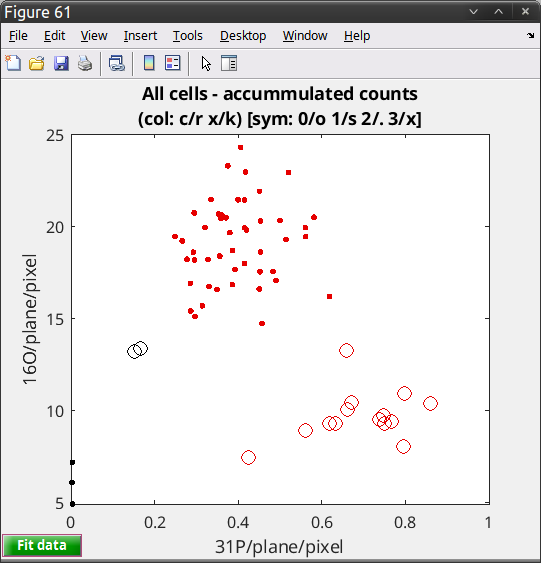
\includegraphics[width=0.4\textwidth]{figs3/LANS-metafile-scatterplot3}
\caption{\label{fig:metafile-scatterplot2}%
Example of a~scatter plot generated by metafile processing after calculating new output variables via metafile auto-processing.}
\end{figure}
